\documentclass[english]{article}

\bibliographystyle{unsrt}

% Section
\newcommand{\secref}[1]{Subsection~\ref{sec.#1}}
\newcommand{\seclabel}[1]{\label{sec.#1}}

% Appendix
\newcommand{\appref}[1]{Appendix~\ref{app.#1}}
\newcommand{\applabel}[1]{\label{app.#1}}

% Table
\newcommand{\tabnum}[1]{\ref{tab.#1}}
\newcommand{\tabref}[1]{Table~\tabnum{#1}}
\newcommand{\tablabel}[1]{\label{tab.#1}}

% Equation
\newcommand{\eqnref}[1]{Equation~\ref{Equations.#1}}
\newcommand{\eqnlabel}[1]{\label{Equations.#1}}

% Figure
\newcommand{\figref}[1]{Figure~\ref{Figures.#1}}
\newcommand{\figlabel}[1]{\label{Figures.#1}}

\newcommand{\easyfig}[4]{
\begin{figure}
\includegraphics[#2]{#1}
\caption{ \figlabel{#3} #4}
\end{figure}}

\newcommand{\dotfig}[4]{
\begin{figure}
\input{#1.tex}
\includegraphics[#2]{#1.ps}
\caption{ \figlabel{#3} #4}
\end{figure}}

\newcommand{\pngfig}[2]{\easyfig{#1.png}{}{#1}{#2}}
\newcommand{\pdffig}[2]{\easyfig{#1-fig.pdf}{}{#1}{#2}}

\newcommand{\widepngfig}[2]{\easyfig{#1.png}{width=\textwidth}{#1}{#2}}
\newcommand{\tallpngfig}[2]{\easyfig{#1.png}{height=.8\textheight}{#1}{#2}}
\newcommand{\widepdffig}[2]{\easyfig{#1-fig.pdf}{width=\textwidth}{#1}{#2}}
\newcommand{\tallpdffig}[2]{\easyfig{#1-fig.pdf}{height=.8\textheight}{#1}{#2}}

\newcommand{\sidewayspngfig}[2]{
\begin{sidewaysfigure}
\includegraphics[width=\textwidth]{#1.png}
\caption{\figlabel{#1} #2}
\end{sidewaysfigure}
}

% ToDo
\newcommand{\needfig}[1]{{\bf Need figure: } #1 }
\newcommand{\needfigref}[1]{Figure~??? [#1] }

\newcommand{\needcite}[1]{[CITE #1]}
\newcommand{\todo}[1]{[TODO: #1]}

% Packages

\usepackage[boxed,noend]{algorithm2e}
\usepackage{graphicx}
\usepackage{psfrag}
\usepackage{url}
\usepackage{amsmath}
\usepackage{amssymb}
\usepackage{color} 
\usepackage{ifthen}
\usepackage{rotating}
\newcommand{\hl}[1]{#1}

\newcommand\semiring{K}
\newcommand\srset{\mathbb{K}}
\newcommand\srplus{\oplus}
\newcommand\srtimes{\otimes}
\newcommand\srplusid{\underline{0}}
\newcommand\srtimesid{\underline{1}}
\newcommand\srsum{\bigoplus}
\newcommand\srprod{\bigotimes}

\newcommand\inalph{\Sigma}
\newcommand\outalph{\Omega}
\newcommand\states{Q}
\newcommand\transitions{E}
\newcommand\initstate{i}
\newcommand\finalstate{f}
\newcommand\emptystring{\epsilon}
\newcommand\maybe[1]{#1 \cup \{ \emptystring \}}

\newcommand\state{q}
\newcommand\trans{t}
\newcommand\src{p}
\newcommand\dest{q}
\newcommand\lab{\ell}
\newcommand\inlab{\lab_i}
\newcommand\outlab{\lab_o}
\newcommand\weight{\mathbb{W}}

\newcommand\somealph{\Gamma}
\newcommand\someseq{\gamma}
\newcommand\midlab{\lab_m}

\newcommand\transcomp{\circ}
\newcommand\transconcat{+}

\newcommand\inseq{\sigma}
\newcommand\outseq{\omega}

\newcommand\kleene[1]{{#1}^{\ast}}
\newcommand\inseqs{\kleene{\inalph}}
\newcommand\outseqs{\kleene{\outalph}}
\newcommand\someseqs{\kleene{\somealph}}

\newcommand\tfunc[1]{\mathbb{#1}}

\newcommand\bigo{{\cal O}}

\newcommand\seqof[1]{\bar{#1}}
\newcommand\sympast{v}
\newcommand\symnext{w}
\newcommand\seqpast{\seqof{\sympast}}
\newcommand\seqnext{\seqof{\symnext}}

\newcommand\nucalph{\somealph_{\mbox{\tiny DNA}}}
\newcommand\sym{x}
\newcommand\comp[1]{\tilde{#1}}
\newcommand\revcomp[1]{\comp{#1}}
\newcommand\ntrans[1]{\hat{#1}}
\newcommand\seqlen[1]{|#1|}
\newcommand\otherseq{\lambda}

\newcommand\kmerlen{{\cal K}}
\newcommand\invreplen{L_{\mbox{\tiny invrep}}}

\newcommand\graph{{\cal G}}
\newcommand\vertices{{\cal V}}
\newcommand\edges{{\cal E}}

\newcommand\debruijngraph{\graph_b}
\newcommand\debruijnvertices{\vertices_b}
\newcommand\debruijnedges{\edges_b}

\newcommand\norepgraph{\graph_r}
\newcommand\norepvertices{\vertices_r}
\newcommand\norepedges{\edges_r}

\newcommand\controlgraph{\graph_c}
\newcommand\controlbridges[1]{\vertices_c(#1)}

\newcommand\prequels{{\cal S}}
\newcommand\stepsto{{\cal L}}

\newcommand\ncontrols{N_c}
\newcommand\controlset{{\cal M}}
\newcommand\controlword{M}

\newcommand\initword{\controlword_i}
\newcommand\finalword{\controlword_f}

\newcommand\initvertex[1]{u^{(#1)}_i}
\newcommand\finalvertex[1]{v^{(#1)}_f}

\newcommand\controlmachine{T_c}

\newcommand\bit[1]{#1_2}
\newcommand\trit[1]{#1_3}
\newcommand\quat[1]{#1_4}
\newcommand\controlsym[1]{{#1}_M}
\newcommand\flushsym{F}

\newcommand\figtrans[2]{T_{\ref{Figures.#1}#2}}
\newcommand\solefigtrans[1]{T_{\ref{Figures.#1}}}

\newcommand\transsingle[2]{T_{#1 \to #2}}
\newcommand\transid[1]{\transsingle{#1}{#1}}
\newcommand\transerase[1]{\transsingle{#1}{\epsilon}}

\newcommand\rbit[1]{#1_{2R}}

\newcommand\hammingthreeone{\figtrans{HammingTransducer}{a}}
\newcommand\hammingsevenfour{\figtrans{HammingTransducer}{b}}

\newcommand\transbintoquat{\figtrans{NaiveDNATransducer}{a}}
\newcommand\transquattodna{\figtrans{NaiveDNATransducer}{b}}
\newcommand\transbintodna{\figtrans{NaiveDNATransducer}{c}}

\newcommand\transdivthree{\figtrans{DivisionByThree}{a}}
\newcommand\transternzeroid{\figtrans{DivisionByThree}{b}}
\newcommand\transternsymid{\figtrans{DivisionByThree}{c}}
\newcommand\transternseqid{\figtrans{DivisionByThree}{d}}
\newcommand\transerasezerobits{\figtrans{DivisionByThree}{e}}
\newcommand\transechodivthree{\figtrans{DivisionByThree}{f}}

\newcommand\transmixed{\figtrans{Converter}{a}}
\newcommand\transflush{\figtrans{Converter}{b}}

\newcommand\transechodivtwo{\figtrans{EvenDivision}{a}}
\newcommand\transechodivfour{\figtrans{EvenDivision}{b}}
\newcommand\transechodivmixed{T_{2 \to 234}}

\newcommand\transpartial{\figtrans{PartialObservation}{c}}

\newcommand\nuc[1]{\mbox{#1}}
\newcommand\nuca{\nuc{A}}
\newcommand\nucc{\nuc{C}}
\newcommand\nucg{\nuc{G}}
\newcommand\nuct{\nuc{T}}

\newcommand\contextlen{L}
\newcommand\seqsyms[2]{\sym_{#1} \ldots \sym_{#2}}
\newcommand\seqpastsyms[2]{\sympast_{#1} \ldots \sympast_{#2}}
\newcommand\seqnextsyms[2]{\symnext_{#1} \ldots \symnext_{#2}}
\newcommand\outsym{y}

\newcommand\param[1]{\mathbb{P}_{#1}}

\newcommand\pnogap{\param{n}}
\newcommand\pdelopen{\param{d}}
\newcommand\ptandup{\param{t}}
\newcommand\pfwddup{\param{f}}
\newcommand\prevdup{\param{r}}

\newcommand\pdelext{\param{x}}
\newcommand\pdelend{\param{e}}

\newcommand\pmatch{\param{m}}
\newcommand\ptransition{\param{i}}
\newcommand\ptransversion{\param{v}}

\newcommand\submat{\param{s}}
\newcommand\lendist{\param{l}}

\newcommand\psub{\submat(\sym,\outsym)}
\newcommand\psubnext[1]{\submat(\symnext_{#1},\outsym)}
\newcommand\psubpast[1]{\submat(\sympast_{#1},\outsym)}
\newcommand\psubcomppast[1]{\submat(\sympast_{#1},\comp{\outsym})}
\newcommand\psubcompnext[1]{\submat(\symnext_{#1},\comp{\outsym})}

\newcommand\plen[1]{\lendist(#1)}

\newcommand\pcont{\pnogap^\ast}

\newcommand\block{\alpha}
\newcommand\srcblock{\block}
\newcommand\destblock{\beta}

\newcommand\blockstate[2]{{#1}_{#2}}
\newcommand\lenstate[3]{\blockstate{#1}{#2}^{(#3)}}

\newcommand\symstate[1]{\blockstate{S}{#1}}
\newcommand\delstate[1]{\blockstate{D}{#1}}
\newcommand\tanstate[2]{\lenstate{T}{#1}{#2}}
\newcommand\fwdstate[2]{\lenstate{F}{#1}{#2}}
\newcommand\revstate[2]{\lenstate{R}{#1}{#2}}

\begin{document}

\newcommand\authorstring{
Ian Holmes$^{1,\ast}$ \\
\textbf{1} Department of Bioengineering, University of California, Berkeley, CA, USA \\
$\ast$ E-mail: ihh@berkeley.edu
}

\newcommand\titlestring{Transducer codes for DNA}
\newcommand\shorttitlestring{Transducer codes for DNA}
\markboth{\shorttitlestring}{\shorttitlestring}
\begin{flushleft}
{\Large \textbf{\titlestring} } \\
\authorstring
\end{flushleft}
%\section{Abstract}
%\paragraph{Keywords:}
%\tableofcontents

\section{Introduction}

Transducers \cite{MohriPereiraRiley2000,WikipediaTransducers}

In bioinformatics:
protein classification \cite{EskinEtAl2000},
phylogenetics \cite{PatenEtAl2008,WestessonEtAlArxiv2012,WestessonEtAl2012},
cancer informatics \cite{SchwarzEtAl2014}

Arithmetic coding \cite{Mackay2003}

DNA storage \cite{ChurchEtAl2012,GoldmanEtAl2013}.
Codes \cite{YazdiEtAl2015}

De Bruijn graphs \cite{DeBruijn1946,PevznerEtAl2001,ZerbinoBirney2008,IqbalEtAl2012}

\section{Methods}

\subsection{Weighted finite-state transducers}

Following \cite{MohriPereiraRiley2000}:
Assume a general semiring
$\semiring=(\srset,\srplus,\srtimes,\srplusid,\srtimesid)$
which for our purposes is typically the probability semiring
$(\Re,+,\times,0,1)$
or the tropical semiring
$(\Re_{+} \cup {\infty},\min,+,\infty,0)$.

A weighted finite-state transducer is defined as a tuple
$T = (\inalph,\outalph,\states,\transitions,\initstate,\finalstate)$
consisting of an input alphabet $\inalph$,
an output alphabet $\outalph$ (both alphabets being finite sets),
a finite set of states $\states$,
a finite set of transitions
$\transitions \subseteq \states \times \maybe{\inalph} \times \maybe{\outalph} \times \srset \times \states$,
an initial state $\initstate \in \states$
and a final state $\finalstate \in \states$.

The transducer $T$ can be thought of as an edge-labelled directed graph
where each state is a vertex
and each transition
$\trans = (\src[\trans],\inlab[\trans],\outlab[\trans],\weight[\trans],\dest[\trans]) \in \transitions$
is an edge from state $\src[\trans]$ to state $\dest[\trans]$
with input label $\inlab[\trans]$,
output label $\outlab[\trans]$
and weight $\weight[\trans]$.
For the figures in this paper,
we adopt the convention that transition labels are annotated as $\inlab{\tt /}\outlab$
(the transition weights for the transducers in the figures are all equal to 1, and are not shown).
\figref{HammingTransducer} shows a transducer that implements the Hamming(3,1) error-correcting code,
\figref{NaiveDNATransducer} shows a transducer that converts a binary string into DNA,
and
\figref{DivisionByThree} shows a transducer that implements division by 3.

A path in $T$ is a series of transitions that form a path in this graph.
The input sequence and output sequence for a path are the concatenation of (respectively)
the input and output labels of the transitions in the path.
The path weight is the $\srtimes$-product of the transition weights.
A successful path is one that starts in $\initstate$ and ends in $\finalstate$.
The transduction weight for a given input sequence $\inseq \in \inseqs$
and output sequence $\outseq \in \outseqs$
is the $\srplus$-sum of all successful paths
having $\inseq$ as the input sequence
and $\outseq$ as the output sequence.
Thus $T$ provides a mapping
$\tfunc{T}:(\kleene{\inalph} \times \kleene{\outalph}) \to \srset$
from sequence-pairs to weights.
We call this mapping $\tfunc{T}$ the transducer function.
For a given pair of sequences $(\inseq,\outseq)$
and a semiring wherein $\srplus$ and $\srtimes$ are amortized-constant resource operations,
it can be evaluated in time $\bigo(|\inseq| \cdot |\outseq| \cdot |\transitions|)$
and memory $\bigo(|\inseq| \cdot |\outseq| \cdot |\states|)$
by dynamic programming,
analogously to the Forward algorithm in the probabilistic semiring
or the Viterbi algorithm in the tropical semiring
\cite{Durbin98}.

A state $\state \in \states$ has past context $\inseqpast$ if every path from $\initstate$ to $\state$ has an input sequence with suffix $\inseqpast$,
and future context $\inseqnext$ if every path from $\state$ to $\finalstate$ has an input sequence with prefix $\inseqnext$.

% This is input context - similarly for output context

\subsection{Transducer composition}

Given transducers
 $R = (\inalph, \somealph, \states_R, \transitions_R, \initstate_R, \finalstate_R)$ and
 $S = (\somealph, \outalph, \states_S, \transitions_S, \initstate_S, \finalstate_S)$
where $R$'s output alphabet is the same as $S$'s input alphabet,
we can readily find a composite transducer
 $T = R \transcomp S = (\inalph, \outalph, \states_T, \transitions_T, \initstate_T, \finalstate_T)$
such that, if $\tfunc{R}$, $\tfunc{S}$ and $\tfunc{T}$ are the corresponding transducer functions,
then
\[
\forall \inseq \in \inseqs, \outseq \in \outseqs:
\quad
\tfunc{T}(\inseq,\outseq) = \srsum_{\someseq \in \someseqs} \tfunc{R}(\inseq,\someseq) \tfunc{R}(\someseq,\outseq)
\]
that is, $T$ models the feeding of $R$'s output into $S$'s input
(and this intermediate sequence is then summed out---i.e. marginalized, if we are in the probabilistic semiring).

Loosely speaking, we can construct $T$ using the following recipe:
\begin{itemize}
\item Each $T$-state corresponds to a pair of $R$- and $S$-states,
so $\state_T = (\state_R, \state_S)$
and $\states_T \subseteq \states_R \times \states_S$.
\item The initial $T$-state $\initstate_T=(\initstate_R,\initstate_S)$ pairs the initial states of $R$ and $S$.
\item The final $T$-state $\finalstate_T=(\finalstate_R,\finalstate_S)$ pairs the final states of $R$ and $S$.
\item $T$-transitions
$\trans_T = ((\src_R,\src_S),\inlab,\outlab,\weight_T,(\dest_R,\dest_S))$
represent (summaries of sets of) synchronized pairs of $R$-transitions
$\trans_R = (\src_R,\inlab,\midlab,\weight_R,\dest_R)$
and $S$-transitions
$\trans_S = (\src_S,\midlab,\outlab,\weight_S,\dest_S)$
which share the same intermediate label $\midlab$.
The composite transition weight $\weight_T$ is the product $\weight_R \srtimes \weight_S$,
or the sum over such products if there are multiple transition-pairs $(\trans_R,\trans_S)$
consistent with a given $\trans_T$
(which, in the probabilistic semiring, is equivalent to marginalizing out $\midlab$).
\item Some additional manipulation is required to synchronize
transitions involving empty input labels (``insertions''),
empty output labels (``deletions''),
or both (``null transitions'').
For example, we can require that $S$-transitions accepting incoming symbols
all originate from ``ready'' states which have no outgoing insertions.
(If $S$ does not comply with this stipulation then we can easily derive a transducer
with the same transducer function $\tfunc{S}$ that does comply.)
\end{itemize}

This algorithm can be made precise enough to automate;
more detailed workings are given elsewhere \cite{PereiraRiley1996,MohriPereiraRiley2000,Holmes2003,Holmes2007,WestessonEtAlArxiv2012,WestessonEtAl2012}.
A simple example of transducer composition is shown in \figref{NaiveDNATransducer}.

\subsection{Transducer concatenation}

Anther operation on transducers that is useful in constructing DNA codes
is concatenation.
Suppose
 $A = (\inalph, \outalph, \states_A, \transitions_A, \initstate_A, \finalstate_A)$ and
 $B = (\inalph, \outalph, \states_B, \transitions_B, \initstate_B, \finalstate_B)$
are transducers with the same input and output alphabets and disjoint state spaces.
The concatenated transducer $C = A \transconcat B$ can be constructed by
taking the union of the state spaces and adding a null ($\epsilon/\epsilon$) unit weight transition
from $\finalstate_A$ to $\initstate_B$.
This models feeding the part of a sequence through $A$ and then feeding the second part through $B$.
Some simple examples of concatenation are shown in \figref{DivisionByThree}.

\subsection{De Bruijn graphs}

The $\kmerlen$-dimensional De Bruijn graph over an alphabet $\somealph$ of cardinality $M$
is a directed graph with $M^\kmerlen$ vertices,
corresponding to all possible $\kmerlen$-symbol strings
$\sym_1 \sym_2 \ldots \sym_\kmerlen \in \somealph^\kmerlen$.
There is an edge $u \to v$ between any two vertices
$u=\sym_1 \sym_2 \ldots \sym_\kmerlen$ and $v=\sym_2 \ldots \sym_\kmerlen \sym_{\kmerlen+1}$
that overlap by $\kmerlen-1$ symbols; this edge is labeled with symbol $\sym_{\kmerlen+1}$ (the last symbol of $v$).
Thus, each vertex has $M$ incoming and $M$ outgoing edges \cite{DeBruijn1946,PevznerEtAl2001}.
Denote this graph by $\debruijngraph = (\debruijnvertices,\debruijnedges)$.

\subsection{A transducer for encoding signals as DNA without short repeats or reserved words}
\seclabel{DeBruijnTransducer}

Let $\nucalph = \{ \mbox{A}, \mbox{C}, \mbox{G}, \mbox{T} \} $ be the nucleotide alphabet and define the complement $\comp{x}$ of a nucleotide symbol $x$,
and the reverse complement $\revcomp{\someseq}$ of a nucleotide sequence $\someseq$, in the usual way.

A direct tandem repeat of length $k$ is a nucleotide sequence followed by an exact copy of itself, $\someseq \someseq$, where the length of each copy is $\seqlen{\someseq}=k$
(note this includes repeated single nucleotides when $k=1$).
Similarly, a direct inverted repeat of length $k$ is a $k$-nucleotide sequence followed by its reverse complement, $\someseq \revcomp{\someseq}$.
A local inverted repeat of length $k$ and separation $l$ is a $k$-nucleotide sequence, followed an $l$-nucleotide sequence, followed by the reverse complement
of the first sequence; that is, $\someseq \otherseq \revcomp{\someseq}$, where $\seqlen{\someseq}=k$ and $\seqlen{\otherseq}=l$.

Start with $\debruijngraph$, the $\kmerlen$-dimensional De Bruijn graph over $\nucalph$.
Delete all nodes corresponding to sequences that contain substrings which are
direct tandem repeats of any length,
direct inverted repeats of length $\geq 2$,
or local inverted repeats of length $\geq \invreplen$ and separation $\geq 2$.
Denote the resulting graph by $\norepgraph = (\norepvertices,\norepedges)$.

Let $A \subset \norepvertices$ be a set of vertices to avoid,
let $D \in A$ be a target vertex,
and denote by $\prequels(D,A,N) \subset \norepvertices$
the set of all vertices
from which there exists a length-$N$ path to $D$
that does not pass through any of the vertices in $A$
(although the path is allowed to originate from one of those vertices).
Define $\stepsto(D,A)$ to be the smallest value of $N$ for which $\prequels(D,A,N) = \norepvertices$,
if such a value of $N$ exists; otherwise, let $\stepsto(D,A)$ be $\infty$.
We can find $\prequels(D,A,N)$ from $\prequels(D,A,N-1)$ by recursive backtracking,
and so determine in $M$ steps whether $\stepsto(D,A) \leq M$.

We now allocate $\ncontrols$ ``control words'': $\kmerlen$-mers that in our transducer
will be unreachable except by specially constructed paths of uniform length.
Specifically, we seek an indexed set of vertices
$\controlset = \{ \controlword_1, \controlword_2 \ldots \controlword_{\ncontrols} \}$
such that $\stepsto(\controlword_n,\controlset) \leq M$ for all $n$
and some value of $M$ (e.g. $M = 2\kmerlen$).
Our implementation finds this list $\controlset$ by brute-force recursive search
and further attempts to maximize the shortest Hamming distance between any two control words in $\controlset$.
Note that there is a ceiling to the number of control words that may be found
for any given value of $\kmerlen$ (and $\invreplen$),
though this ceiling grows rather rapidly with $\kmerlen$.
In practice we only need a few control words for most purposes.

Having designated some $\kmerlen$-mers as control words via analysis of $\norepgraph$,
we now construct a new graph $\controlgraph$
in which the control words are unreachable from the other words
except by paths that we construct.
Starting with graph $\norepgraph$, delete all incoming transitions to control words $\controlword_n \in \controlset$,
rendering them unreachable,
and prune the graph of any other nodes that become unreachable as a result.
Next, for every control word $\controlword_n \in \controlset$
and every path length $1 \leq k < \stepsto(\controlword_n,\controlset)$,
we create a new vertex set $\controlbridges{n,k}$
with a one-to-one correspondence to $\prequels(\controlword_n,\controlset,k)$.
We connect the newly-added vertices such that there is an edge from
$u \in \controlbridges{n,k}$ to $v \in \controlbridges{n,k-1}$
for every corresponding edge $(u',v') \in \norepedges$ between
$u' \in \prequels(\controlword_n,\controlset,k)$
and
$v' \in \prequels(\controlword_n,\controlset,k-1)$.
We also add edges from
$u \in \norepvertices$ to $v \in \controlbridges{n,\stepsto(\controlword_n,\controlset)}$
for the first steps in the paths to control words,
as well as edges from
$u \in \controlbridges{n,1}$ to $\controlword$
for the final steps.
In each case the newly-added edge is copied from a corresponding edge in $\norepedges$
and inherits the same edge label.

It can be useful to force the transducer to start with a particular control word $\initword$
and finish with another (or the same) control word $\finalword$.
To guarantee this we can add a chain of initial vertices and edges leading from source vertex to the initial control word,
$\initvertex{0} \to \initvertex{1} \to \initvertex{2} \to \ldots \to \initvertex{\kmerlen-1} \to \initword$,
with each transition labeled with consecutive symbols from the initial control word.
We also need to add a transition from the final control word to the final state.
(If the start and end control words are the same, then this vertex should be duplicated to prevent cycles.)

We have now constructed the graph $\controlgraph$ from which our transducer $\controlmachine$
is derived via the following recipe:
\begin{itemize}
\item Every vertex in $\controlgraph$ is a state in $\controlmachine$.
The initial and final vertices of $\controlgraph$ are the initial and final states of $\controlmachine$.
\item Every edge in $\controlgraph$ is a unit-weight transition in $\controlmachine$.
The output label of the transition is the label of the edge.
\item The input label of each transition is determined as follows:
\begin{itemize}
\item For states in $\norepvertices$ with two outgoing transitions to other states in $\norepvertices$, those transitions are input-labeled with the binary digits $\bit{0}$ and $\bit{1}$.
\item For states in $\norepvertices$ with three outgoing transitions to other states in $\norepvertices$, those transitions are input-labeled with the trinary digits $\trit{0}$, $\trit{1}$ and $\trit{2}$.
\item For states in $\norepvertices$ with four outgoing transitions to other states in $\norepvertices$, those transitions are input-labeled with the quaternary digits $\quat{0}$, $\quat{1}$, $\quat{2}$ and $\quat{3}$.
\item Transitions from states in $\norepvertices$ to states in $\controlbridges{n,\stepsto(\controlword_n,\controlset)}$,
which begin a path to the $n$'th control word $\controlword_n$,
are input-labeled with the special control digit $\controlsym{n}$.
\item All other transitions have input label $\emptystring$.
\end{itemize}
\end{itemize}

Thus, the input alphabet of $\controlmachine$
is $\{ \bit{0}, \bit{1},
       \trit{0}, \trit{1}, \trit{2},
       \quat{0}, \quat{1}, \quat{2}, \quat{3},
       \controlsym{1} \ldots \controlsym{\ncontrols} \}$.

\figref{DNAStore} illustrates some of the code transducers that are generated by this procedure for the simplest case $\kmerlen=2$.
       
\subsection{The delayed transducer}

By virtue of being derived from the De Bruijn graph, most of the states in the transducer of \secref{DeBruijnTransducer}
have $\kmerlen$ nucleotides of past context.
% This confuses input and output context - fix!
We can transform this transducer into an equivalent one wherein most of the states have
$\kmerlen/2$ nucleotides of past context
and $\kmerlen/2$ nucleotides of future context.

This can be a convenient way to think about context, for the purpose of modeling errors in DNA replication and sequencing.
Common decoding and replication errors include local tandem and inverted duplications, as well as context-dependent substitutions.
These can occur on either strand of and therefore (depending on the representation) may be best represented as depending
on future context as well as past context.

The transformation requires that the output sequence of all successful paths through the transducer
begin with a particular $\kmerlen$-mer and end with a particular $\kmerlen$-mer,
which can be ensured using the method described in \secref{DeBruijnTransducer}.

Let $\someseq = \inseqpast(\state)$ be the past context for a given state $\state$.
All of the transitions $\trans$ into $\state$ have the same input label $\inlab[\trans] \equiv \inlab[\state]$,
which corresponds to the most recent nucleotide of context for that state,
i.e. the $\kmerlen$'th symbol of $\someseq$.
If, instead, we set $\inlab[\trans]$ to be the $(\kmerlen/2)$'th symbol of $\someseq$
for all transitions into $\state$, then we have effectively delayed all output by $\kmerlen/2$ symbols.
We can now predict the next $\kmerlen/2$ symbols in the output sequence for the path from a state,
so we have traded $\kmerlen/2$ of past context for $\kmerlen/2$ of future context.

We need to add $\kmerlen/2$ extra padding states after (what was originally) the final state,
with a chain of transitions that flushes out the final $\kmerlen/2$ delayed output symbols.
Conversely, the first $\kmerlen/2$ transitions from the initial state will, after the transformation,
be null transitions (with both input and output labels equal to $\emptystring$),
so these transitions and the corresponding states can be deleted.



\subsection{A transducer that converts a binary sequence into a mixture of binary, trinary and quaternary}

Not every state accepts symbols of the same radix...

We need a converter that can context-switch between binary, trinary, and quaternary...

\figref{Converter}...

\subsection{Making the decoder robust to substitutions, local tandem and inverted duplications, and other indels}

Error-modeling transducer...
% Use future context to reduce # of states needed for invreps?


\newpage
\section{Figures}

\newpage
\begin{figure}
\begin{tabular}{ll}
(a) \includedot{hamming31}{width=.45\textwidth}
&
(b) \includegraphics[width=.45\textwidth]{hamming74.ps}
\end{tabular}
\caption{ \figlabel{HammingTransducer}
Left (a):
A transducer that implements the Hamming(3,1) error-correcting code
(which simply repeats every bit three times).
S is both the initial state and the final state.
Right (b):
A transducer that implements the Hamming(7,4) error-correcting code,
with four data bits and three parity bits.
Due to the large number of states, the state names have been omitted from this diagram,
as have the $\epsilon$ labels for empty inputs or outputs.
}
\end{figure}

\newpage
\begin{figure}
\begin{tabular}{lll}
(a) \includedot{binary2quaternary}{width=.3\textwidth}
&
(b) \includedot{quaternary2dna}{width=.3\textwidth}
&
(c) \includedot{binary2dna}{width=.3\textwidth}
\end{tabular}
\caption{
\figlabel{NaiveDNATransducer}
Left (a):
Transducer $\transbintoquat$ converts a binary input string (presented least-significant digit first) into a quaternary input string.
Binary input digits are written showing the radix-2 suffix ($\bit{0}$, $\bit{1}$),
while quaternary output digits are written showing the radix-4 suffix, ($\quat{0}$, $\quat{1}$, $\quat{2}$, $\quat{3}$).
The initial state is S and the final state is E.
Middle (b):
Transducer $\transquattodna$ converts a quaternary input string into a DNA string.
Right (c):
Transducer $\transbintoquat \transcomp \transquattodna$
converts a binary input string to DNA.
This machine is obtained by composing the ``binary to quaternary'' transducer ($\transbintoquat$) with the ``quaternary to DNA'' transducer ($\transquattodna$).
}
\end{figure}

\newpage
\begin{figure}
\begin{tabular}{lcr}
\multicolumn{3}{c}{}
(a) \includedot{divisionby3}{width=\textwidth}
\\
(b) \includedot{trinary0}{width=.2\textwidth}
&
(c) \includedot{trinaryunion}{width=.2\textwidth}
&
(d) \includedot{trinaryid}{width=.2\textwidth}
\\
(e) \includedot{binaryeraser}{width=.15\textwidth}
&
(f) \includedot{trinaryonly}{width=.45\textwidth}
\\
\multicolumn{3}{c}{}
(g) \includedot{binary2trinary}{width=\textwidth}
\end{tabular}
\caption{
\figlabel{DivisionByThree}
Top row (a):
Transducer $\transdivthree$ implements the operation ``division by three''.
The machine accepts as its input sequence a binary number representing the divisor, which must be presented most significant bit first.
It outputs the quotient (as a similar binary sequence) followed by the remainder (as a trinary digit).
The machine's state encodes the current remainder at any stage during the division.
Binary digits are written as $(\bit{0}, \bit{1})$
and trinary digits as $(\trit{0}, \trit{1}, \trit{2})$.
Second row (b,c,d):
Union and Kleene closure.
Left of second row (b):
The transducer $\transid(\sym)$ echoes a single specified digit from input to output; in this case, $\sym=\trit{0}$.
Center of second row (c):
The transducer union $\transid(\trit{0}) \cup \transid(\trit{1}) \cup \transid(\trit{2})$, which echoes any of the three trinary digits.
Right of second row (d):
The transducer $\transternid$ echoes any number of trinary digits, and may be written as
the Kleene closure $\transternid = \left( \transid(\trit{0}) \cup \transid(\trit{1}) \cup \transid(\trit{2}) \right)^\ast$.
This implements the identity operation for trinary sequences.
Third row (e,f):
Some further simple transducers that are useful in the implementation of ``binary to trinary conversion'',
also illustrating transducer concatenation.
Left of middle row (e):
Transducer $\transerase(\sym)$ erases a given symbol (i.e accepts that symbol on the input but outputs the empty string); in this case, the erased symbol is the binary zero, $\bit{0}$.
Right of middle row (f):
Transducer $\transternid \transconcat \transerase(\bit{0})^\ast$ is the concatenation of the trinary identity (d) with the Kleene closure of the binary-zero eraser (e).
Bottom row (g):
Transducer $\transternid \transconcat \transdivthree$
is a concatentation of the ``trinary identity'' transducer (d)
with the ``division by three'' transducer (a).
It uses the S and T states from $\transternid$ and the $0$, $1$, $10$ and E states from $\transdivthree$.
By composing a series of $N$ transducers of this form, along with a final step that removes the remaining binary digit,
we can convert a binary number into $N$ trinary digits \cite{MartinsFerreira2012}.
For example, to output three trinary digits, we could use the composed transducer
$ \transdivthree \transcomp (\transternid \transconcat \transdivthree) \transcomp (\transternid \transconcat \transdivthree) \transcomp (\transternid \transconcat \transerase(\bit{0})^\ast)$.
}
\end{figure}

\newpage
\begin{figure}
\begin{tabular}{ll}
  (a) \includedot{converter}{width=.5\textwidth}
&
  (b) \includedot{flush8}{width=.5\textwidth}
  \end{tabular}
\caption{
\figlabel{Converter}
Left (a):
Transducer $\transmixed$ converts an input sequence of binary digits ($\bit{0},\bit{1}$),
optionally interleaved with
control symbols ($\controlsym{n}$)
and flush symbols ($\flushsym$),
into a mixed output of binary digits,
trinary digits ($\trit{0},\trit{1},\trit{2}$),
quaternary digits ($\quat{0},\quat{1},\quat{2},\quat{3}$),
and control symbols, which are simply echoed to the output;
the flush symbol is used to drive the machine into a state (T) where it can accept control symbols.
The conversion is suboptimal in that trinary digits (trits) on average encode
1.5 input bits, slightly less than the theoretical maximum of $\log_2(3) \simeq 1.58$ bits.
State S is both the initial state and the final state.
Right (b):
Transducer $\transflush$ copies input bits to the output, sending a flush symbol after every 8-bit byte.
Accurate decoding of the output sequence from $\transmixed$ requires that the decoder
knows at what points in the sequence flush symbols have been encoded.
This synchronization can be formalized by using $\transflush \transcomp \transmixed$,
i.e. passing the input sequence through the ``flush every 8 bits'' transducer
before feeding it to the ``convert to binary/trinary/quaternary'' transducer.
In this model, bytes cannot be split up; a control symbol can only be sent before or after a byte,
and an input bitstream that has a control symbol partway through an 8-bit block
will have no successful path through the transducer.
}
\end{figure}

\newpage
\begin{figure}
\begin{tabular}{ll}
  (a) \includedot{divisionby2}{width=.5\textwidth}
&
  (b) \includedot{divisionby4}{width=.5\textwidth}
  \end{tabular}
\caption{
\figlabel{EvenDivision}
Left (a):
Transducer $\transdivtwo$ divides a binary input by two,
outputting quotient and remainder in binary.
To distinguish quotient from remainder,
the remainder is expressed using a different alphabet $\{ \rbit{0}, \rbit{1} \}$.
The quotient is expressed using the same alphabet as the divisor $\{ \bit{0}, \bit{1} \}$.
Right (b):
Transducer $\transdivfour$ divides a binary input by two,
outputting quotient in binary followed by remainder in quaternary.
}
\end{figure}

\newpage
\begin{figure}
\begin{tabular}{ccc}
(a) \includedot{dna2full}{width=.3\textwidth}
&
(b) \includedot{dna2start}{width=.3\textwidth}
&
(c) \includedot{dna2startend}{width=.3\textwidth}
\\
(d) \includedot{dna2norep}{width=.3\textwidth}
&
(e) \includedot{dna2startnorep}{width=.3\textwidth}
&
(f) \includedot{dna2startendnorep}{width=.4\textwidth}
\end{tabular}
\caption{
  \figlabel{DNAStore}
  Transducers generated using the method of \secref{DeBruijnTransducer} with $\kmerlen=2$.
  These codes are all fundamentally based on the 2-dimensional De Bruijn graph
  from which vertices are duplicated, deleted and added to arrive at a transition graph with the required properties.
  Top row (a,b,c): codes in which dinucleotide repeats are not prohibited.
  Bottom row (d,e,f): codes in which dinucleotide repeats are not prohibited.
  Left column (a,d): codes in which there are no reserved control words, so the machine start and end in arbitrary states.
  Central column (b,e): codes in which there is one reserved control word, which only ever appears once, at the start of the encoded DNA sequence.
  Right-hand column (c,f): codes in which there is one reserved control word, which only ever appears twice: once at the start of the encoded DNA sequence and once at the end.
  The leftmost machine in the top row (a) is similar to $\transbintoquat \transcomp \transquattodna$ of \figref{NaiveDNATransducer}(c),
  while the leftmost machine in the bottom row (d) is similar to the trinary code of \cite{GoldmanEtAl2013}.
  {\bf Key:}
  Transition label annotations have been omitted from this diagram to reduce clutter.
  Instead, they may be deduced from the node and edge shapes, as follows:
  Bold-line transitions from rectangular states encode quaternary input digits.
  Solid-line transitions from triangular states encode trinary input digits.
  Dashed-line transitions from double-circle states encode binary input digits.
  Dotted-line transitions do not encode input digits;
  states that can only be exited via these transitions are shown as rectangles.
  Transitions that encode input digits have empty circles at the source end;
  transitions that encode output digits have filled arrowheads at the destination end.
}
\end{figure}

\newpage
\bibliography{trans}



\end{document}
